\subsubsection{Word representation}
\label{sub:word_representation}

The starting point for most NLP related tasks lies within the preprocessing of the textual input data. These must first be converted into a semantically meaningful numerical representation to allow for effective computation. The simplest way to represent a word numerically is by treating words as \textit{one-hot} vectors. Using this format, one word is encoded into an $ n $-dimensional vector of numbers where $ n $ is the vocabulary size and each entry takes on the value $ 0 $ except for the one that corresponds to the indexed word which takes on the value $ 1 $. This process generates very sparse feature vectors for each input word, which is no problem for simple classification tasks but is unsuitable for larger problems as the dimension size increases for each word added to the vocabulary. Another issue of one-hot vectors is the fact that these representations hold no notion of similarity: If we take a look at the representations for the words “plane“ and “airplane“ we would get two orthogonal vectors, just like any two vectors in the whole vocabulary. This poses a problem as every word's similarity to other words is the same and we can not encapsulate the meaning of the word. Yoav Goldberg writes in his primer on neural networks for language processing that one-hot vectors should only be considered for problems where the model has only a small amount of input features, the inputs do not have to share model parameters and where there is a lot of data to learn from~\footcite{DBLP:journals/corr/Goldberg15c}.

Otherwise, the currently dominant approach in the field is to use word embeddings as feature vectors. Word embeddings follow the so-called “distributional semantics“, which state that a word's meaning is given by the words that tend to occur in a similar context. This idea of context-dependent nature of meaning was first introduced by English linguist J.R. Firth~\footnote{\url{https://web.stanford.edu/class/linguist236/materials/ling236-handout-05-09-vsm.pdf}} with the famous quote:

\begin{quote}
  You shall know a word by the company it keeps.
\end{quote}

Following this idea we represent each word by a distribution of weights across many dimensions. Now, instead of having a one-to-one mapping between an element in the vector and a word, the representation of a word is spread across all of the entries in the vector, and each element in the vector contributes to the definition of many words. Having this new form of word vectors allows us to capture meaningful semantic and syntactic regularities between words expressively. A simple way to illustrate this is depicted in figure~\ref{fig:word2vec_king_queen_composition}. \\
Here, our word vectors contain the knowledge that the difference between a “king“ and a “queen“ primarily lies within the gender of a person. Thus, if we subtract the word vector of “man“ from “king“ and we add the word vector of “woman“ we get a word vector that is very similar to the one of “queen“.

\begin{figure}[h]
  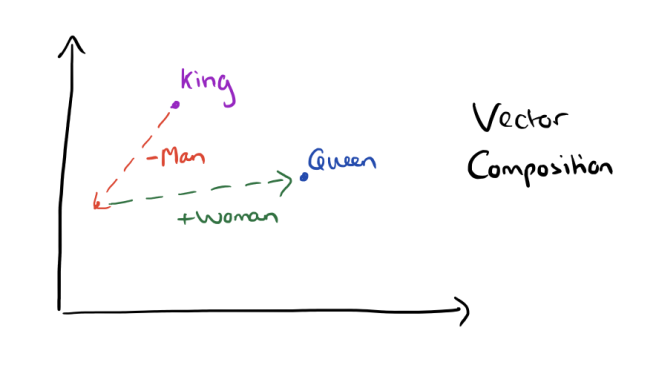
\includegraphics[height=5cm]{img/word2vec-king-queen-composition}
  \caption{Word2vec king queen composition}
\label{fig:word2vec_king_queen_composition}
\end{figure}

The most famous realization of these embeddings was introduced by the researchers of Google around Tomas Mikolov in their paper “Distributed Representations of Words and Phrases and their Compositionality“~\footcite{DBLP:journals/corr/MikolovSCCD13}. Hereafter, their proposed approach, Word2Vec, along with their used notation will briefly be presented, as its core ideas are found throughout other popular word embedding frameworks as well. \\
Given a sequence of training words $ w_1, w_2, \dots, w_T $, the objective (paragraph~\ref{par:cost_function}) is to minimize the average negative log-likelihood
\begin{equation}
	\label{eqn:skip_gram_objective_function}
	J(\theta) = - \frac{1}{T} \sum_{t=1}^{T} \sum_{\substack{-m \leq j \leq m \\ j \neq 0}} \text{log} \ P(w_{t+j} | w_t; \theta)
\end{equation}
where $ m $ is the fixed window size containing the context words around the center word $ w_j $. Enlarging this window size results in more training examples and can lead to a higher accuracy, at the expense of training time. In order to compute the term $ P(w_{t+j} | w_t; \theta) $ a regular softmax function (ch 3.3.3 [HARDCODED, ref to softmax function]) can be applied
\begin{equation}
	\label{eqn:skip_gram_conditional_probability}
	P(o | c) = \frac{\text{exp} \ (u_{o}^{T} v_{c})}{\sum_{w \in V} \text{exp} \ (u_{w}^{T} v_c)}
\end{equation}
where we use two vectors per word $ w $: $ v_w $ when $ w $ is a center word and $ u_w $ when $ w $ is a context word. Optimizing the objective function results in high-quality distributed vector representations. It should be noted that for computational efficiency modified versions of these functions such as negative sampling or hierarchical softmax are used, as the presented ones do not scale well.

Even though word2vec embeddings are a powerful representation they do face certain limitations, which is why scientists at Stanford University took it upon themselves to create an improved variant called GloVe~\footcite{pennington-etal-2014-glove}. While word2vec ignores that some context words appear more often than others, GloVe stresses the importance of frequencies of co-occurrences and that these should not be “wasted“ as additional training examples. Therefore, GloVe builds word embeddings in a way that a combination of word vectors relates directly to the probability of these words' co-occurrence in the corpus. \\
Another alternative to word2vec is \textit{fasttext} by Facebook, which generates word vectors that generalize better, need less training data and can be trained “on more than one billion words in less than ten minutes using a standard multicore CPU, and classify half a million sentences among 312K classes in less than a minute“ according to the authors~\footcite{DBLP:journals/corr/JoulinGBM16}. FastText also takes word parts into account, i.e. FastText not only stays on a word level of depth but also goes into the character level.
